\documentclass{article}
\usepackage[margin=1in]{geometry}
\usepackage{amsmath,amsfonts,amssymb,amsthm}
\usepackage{graphicx}
\usepackage{enumitem}
\usepackage{authblk}
\usepackage{hyperref}
\usepackage{xcolor}
\usepackage{float}
\usepackage{caption}
\usepackage{subcaption}
\usepackage{booktabs}
\usepackage{multirow}
\usepackage{array}
\usepackage{tikz}
\usetikzlibrary{positioning}
\usepackage{listings}
%\usepackage{microtype}
\usepackage{mathtools}
\usepackage{pgfplots}
\usepackage{siunitx}
\usepackage{amssymb}
\pgfplotsset{compat=1.18}

\hypersetup{
    colorlinks=true,
    linkcolor=blue,
    filecolor=magenta,
    urlcolor=cyan,
    citecolor=blue,
}

\lstdefinestyle{py}{
  language=Python,
  basicstyle=\ttfamily\small,
  keywordstyle=\color{blue}\bfseries,
  commentstyle=\color{teal!60!black}\itshape,
  stringstyle=\color{red!60!black},
  showstringspaces=false,
  frame=tb,
  numbers=left,
  numberstyle=\tiny\color{gray},
  breaklines=true,
  tabsize=2,
  keepspaces=true
}

\newtheorem{proposition}{Proposition}
\newtheorem{assumption}{Assumption}
\newtheorem{lemma}{Lemma}
\newtheorem{definition}{Definition}
\newtheorem{theorem}{Theorem}
\newtheorem{corollary}{Corollary}

\title{Verifiable Structured Generation in LLMs via Tokenizer-Aware Constraints, Proper Masked Training, and Bounded Repair}

\author[1]{David Xu}
\affil[1]{China Mobile Research Institute}
\date{}

\begin{document}
\maketitle

\begin{abstract}
We present OIP-CAD, a verification-first framework for structured generation in large language models (LLMs). OIP-CAD integrates: (i) tokenizer-aware safety using a formal boundary model, deterministic BPE/WordPiece/Unigram contracts with proofs and detectors that include Unicode/normalization edge cases and a versioned self-test manifest with conservative fallbacks; (ii) masked-logit training with a complete proof of strict properness as $B\to\infty$, explicit finite-$B$ leakage bounds and sensitivity, and an adaptive masking schedule that preserves calibration under mixture training; (iii) deterministic, bounded-latency minimal-edit repair via anytime A* (ARA*) with a max-combination of consistent admissible heuristics and an ILP fallback with stated total unimodularity (TU) conditions and diagnostics; and (iv) ontology-initialized prefixes (OIP) trained with InfoNCE that are provably safe under mask dominance and constrained by a KL trust region, with ablations and a process reward model (PRM) integration.

Tokenizer theory: We formalize protected boundaries as regular languages over bytes and prove a 3-token greedy locality lemma for BPE/WordPiece under a total merge order with deterministic tie-breaking. We provide a full proof and quantify detector complexity and false negatives across horizons $L\in\{3,4,5\}$ with worst-case instances necessitating $L=4$. We release a runtime self-test that caches verdicts per tokenizer version and escalates policies when assumptions fail. Cross-lingual stress tests cover virama/ZWJ shaping and emoji sequences across normalization forms.

Training theory: We prove strict properness of masked cross-entropy on the restricted simplex for any temperature and label smoothing as $B\to\infty$, derive finite-$B$ leakage bounds with explicit partition functions, and empirically validate tightness across $(K,k,T,\alpha,B,\Delta)$. We provide an adaptive schedule that maintains illegal mass below a configured threshold with margin and report calibration trade-offs across mixture weights.

Repair: We define automaton-, type-, and structure-based heuristics, prove admissibility/consistency on the $\epsilon$-closed product graph, and report certificates and optimality gaps under ARA*. An ILP fallback is specified with variables, constraints, TU conditions, and non-TU diagnostics.

Composition: We formalize composition of subsequential transducers with FSAs/PDAs, give a worked example, state sufficient conditions for uniqueness, and provide an ambiguity diagnostic and policy.

Evaluation emphasizes safety-efficiency Pareto trade-offs and detailed ablations on JSON/KG, Spider, and code (HumanEval/MBPP/MultiPL-E). We include detector triggers, fallback/repair rates, Unicode robustness, calibration curves with CIs, scalability curves, and deterministic harnessing. OIP-CAD delivers lower unsafe emissions with competitive or better acceptance, strong downstream utility, and verifiable tokenizer safety.
\end{abstract}

\section*{Glossary (pruned)}
- FSA/PDA: Finite-State/Pushdown Automaton.
- OIP: Ontology-Initialized Prefixes.
- CAD: Constraint-Aware Decoding.
- ARA*: Anytime weighted A* with decreasing weights.
- PRM: Process Reward Model.

\section*{Symbols and Notation}
- $\mathcal{U}$: byte alphabet; $\Sigma$: tokenizer tokens; $\Gamma$: grammar/output symbols.
- $T$: temperature; $\eta$: label smoothing; $\alpha,B$: mask parameters.
- $K=|\Sigma|$, $k=|\mathcal{S}_t|$: vocabulary and legal-set sizes.
- $\Delta$: max logit margin between best legal vs best illegal.
- $L$: locality horizon; $M$: number of BPE merges; $G_\tau$: Merge-DAG.
- Types: a finite set $\mathsf{T}$ of semantic classes (e.g., number, string, identifier) mapped to token subsets via a predicate $P:\Sigma\to 2^{\mathsf{T}}$.

\begin{figure}[H]
\centering
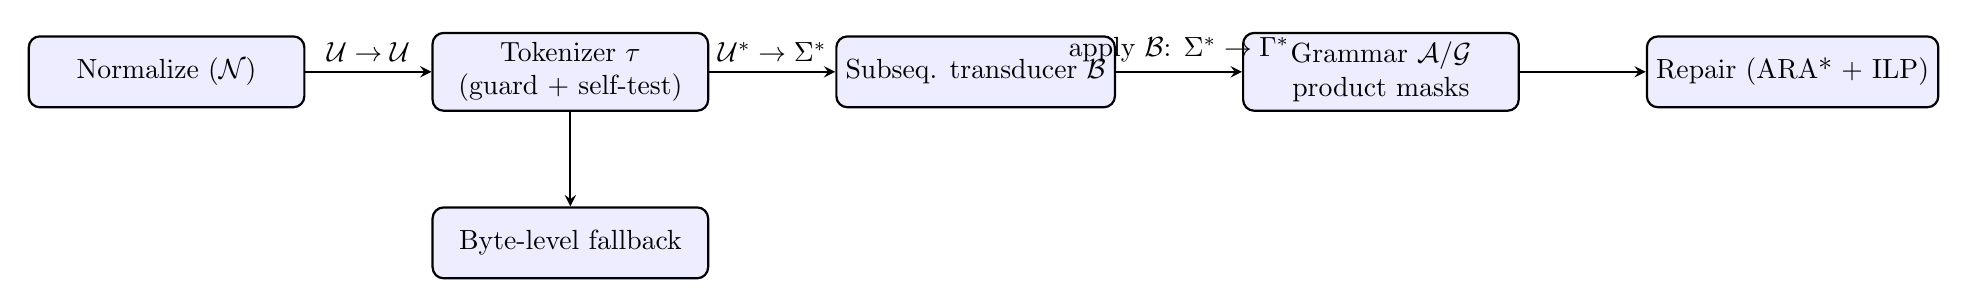
\begin{tikzpicture}[node distance=1.2cm,>=stealth,thick]
\tikzstyle{block}=[rectangle,rounded corners,draw=black,fill=blue!7,align=center,minimum width=3.5cm,minimum height=0.9cm]
\node[block] (norm) {Normalize ($\mathcal{N}$)};
\node[block, right=1.6cm of norm] (tok) {Tokenizer $\tau$\\(guard + self-test)};
\node[block, right=1.6cm of tok] (trans) {Subseq. transducer $\mathcal{B}$};
\node[block, right=1.6cm of trans] (auto) {Grammar $\mathcal{A}/\mathcal{G}$\\product masks};
\node[block, below=1.2cm of tok] (byte) {Byte-level fallback};
\node[block, right=1.6cm of auto] (repair) {Repair (ARA* + ILP)};
\draw[->] (norm) -- node[above]{$\mathcal{U}\to\mathcal{U}$} (tok);
\draw[->] (tok) -- node[above]{$\mathcal{U}^\ast\to\Sigma^\ast$} (trans);
\draw[->] (trans) -- node[above]{apply $\mathcal{B}$: $\Sigma^\ast\to\Gamma^\ast$} (auto);
\draw[->] (tok) -- (byte);
\draw[->] (auto) -- (repair);
\end{tikzpicture}
\caption{Flow: normalization, tokenizer with guard/self-test, subsequential transducer, and automata products producing masks; byte-level fallback and repair are safety refinements.}
\end{figure}

\section{Introduction and Design Decisions}
LLMs must emit structured artifacts accepted by schemas, parsers, and compilers. Constrained decoding tightly couples to subword tokenizers and recursive grammars. OIP-CAD adopts a safety-first contract:
- Tokenizer guard: a formal boundary model with detectors and a runtime self-test manifest; ambiguous cases trigger conservative fallbacks (byte-level spans).
- Masked training: align the model to constrained supports with soft masks; control leakage via adaptive schedules; mix with unconstrained batches for calibration.
- Constrained decoding: deterministic masks from FSA/PDA products; no illegal token is committed.
- Multi-fidelity backoff and repair: shadow byte-level backoff and minimal-edit repair (ARA* + ILP) within latency SLAs.
- OIP + PRM: ontology-grounded prefixes and process rewards, both strictly post-mask to preserve safety.

Our design emphasizes verifiability: each component has explicit contracts, testable assumptions, and measurable certificates. We prioritize monotonic safety (no “unsafe success”) and deterministic execution where possible to improve reproducibility.

\section{Preliminaries, Assumptions, and Safety Invariant}
Bytes $\mathcal{U}$, tokens $\Sigma$, outputs $\Gamma$; tokenizer $\tau:\mathcal{U}^\ast\to\Sigma^\ast$; subsequential transducer $\mathcal{B}:\Sigma^\ast\to\Gamma^\ast$; grammar $\mathcal{A}$ (FSA) or $\mathcal{G}$ (PDA). Validators may be stricter than $\mathcal{A}/\mathcal{G}$.

\begin{definition}[Protected boundary]
A protected boundary is a regular language $\mathcal{R}\subseteq\mathcal{U}^\ast$ recognized by a DFA, typically a singleton byte string $b\in\mathcal{U}^\ast$ (e.g., quotes, sentinels) or an equivalence class under normalization $\mathcal{N}$. Let $\mathsf{Tok}(b)\subseteq\Sigma$ be the set of token ids whose byte realization equals $b$.
\end{definition}

\begin{definition}[Atomicity and non-creation]
Given $x\in\mathcal{U}^\ast$ and its tokenization $\tau(x)=t_1\dots t_n$, a boundary $b\in\mathcal{R}$ is atomic if any occurrence of $b$ in $x$ is realized by a contiguous sub-sequence of tokens whose concatenated bytes equal $b$, with at least one token in $\mathsf{Tok}(b)$ when defined. Non-creation means no greedy merge sequence can introduce a contiguous byte span equal to $b$ where none existed in the raw bytes.
\end{definition}

\begin{assumption}[Tokenizer model and implementation]\label{assump:tok}
(i) Greedy merges apply to strictly adjacent pairs under a total order over pairs; (ii) tie-breaking is deterministic and stable across runs; (iii) merge ranking is stable within a version; (iv) special tokens are verbatim, excluded from merges; (v) declared normalization $\mathcal{N}$ precedes tokenization; (vi) no undocumented filtering of Unicode controls; (vii) pre-tokenization behavior is documented (e.g., added\_prefix\_space); (viii) for WordPiece, prefix/suffix markers are part of tokens and merges respect word boundaries.
\end{assumption}

\begin{definition}[Safety invariant]
At every decoding step, the committed prefix maps via $\mathcal{B}$ into a string in $\mathcal{L}(\mathcal{A})$ or $\mathcal{L}(\mathcal{G})$ and satisfies type predicates. External validators may be stricter; disagreement triggers repair or abstention. Fidelity switches preserve this invariant by pre/post-conditions and rollback.
\end{definition}

\begin{definition}[No-valid-token condition]
At step $t$ in product state $s_t$, the legal set $\mathcal{S}(s_t)=\{v\in\Sigma:\delta_{\mathcal{P}}(s_t,v)\text{ defined}\}$ is empty. The system must switch fidelity (shadow byte-level backoff or repair) or abstain. Example: JSON expects a closing quote, but tokenizer cannot emit it safely due to an unsafe boundary; detector triggers byte-level backoff to emit bytes until resynchronization.
\end{definition}

\section{Tokenizer Safety: Theory, Manifest, and Detection}\label{sec:tokenizers}
\subsection{Greedy locality for BPE/WordPiece}
\begin{lemma}[3-token greedy locality]\label{lem:local}
Under Assumption~\ref{assump:tok}, let $b\in\mathcal{R}$ be a fixed boundary byte string, and let $x\in\mathcal{U}^\ast$ with $\tau(x)=t_1\dots t_n$. Consider any greedy merge schedule consistent with the total pair order. Any merge that (a) destroys an existing contiguous occurrence of $b$ (by absorbing it into a larger byte span) or (b) creates a new contiguous occurrence of $b$ must involve two tokens whose byte spans lie within the concatenation of at most three consecutive tokens: the token covering the left context adjacent to $b$, the token(s) covering $b$ (if present), and the token covering the right context adjacent to $b$. Therefore, changes to the presence or atomicity of $b$ are detectable within a 3-token window.
\end{lemma}

\begin{proof}
We formalize a greedy schedule as a sequence of reductions on a string of token ids, where each step replaces adjacent pair $(u,v)$ by a merged id $w$ if ranked highest among all currently available adjacent pairs. Let positions be indexed by current token boundaries. Let $I$ denote the minimal interval of positions covering: (i) the left neighbor of $b$, (ii) the tokens whose concatenated bytes equal $b$ if $b$ is already present, and (iii) the right neighbor of $b$; when $b$ is absent, (ii) is the boundary between the two tokens whose concatenation could equal $b$ after merges.

We show by induction that any merge outside $I$ commutes with any sequence of merges inside $I$ with respect to the predicate “there exists a contiguous occurrence of $b$ in the current byte string.” First, merges outside $I$ do not alter bytes inside $I$, as merges only replace adjacent tokens by their concatenation and do not cross token boundaries. Second, the total order on pairs ensures that if a higher-ranked external pair preempts a local pair, we can swap their order without changing the existence of $b$: external merges change neither the local adjacency of token boundaries nor the byte substrings inside $I$. This yields a Church–Rosser-style confluence for the predicate on the subset of reductions that affect $I$. 

Creation: Suppose a merge schedule first creates an occurrence of $b$ at some step. Let this be the earliest step where $b$ appears. The merged pair at that step must straddle the would-be boundary between two adjacent tokens whose concatenation equals $b$; both lie within $I$ by construction, hence within at most three consecutive tokens.

Destruction: Suppose a merge schedule first destroys an existing occurrence of $b$ at some step, by merging $b$ with an adjacent neighbor. The merged pair must include the token span equal to $b$ and one of its immediate neighbors; both lie within $I$. WordPiece respects subword boundary markers; merges remain adjacent within words, so the same locality applies. Deterministic tie-breaking preserves the total order; if ties are non-deterministic, they can be adversarial and are handled by elevating $L$ and exhaustively testing short contexts (Appendix~\ref{app:locality}).
\end{proof}

\begin{theorem}[Boundary preservation under locality]\label{thm:bpe}
Under Assumption~\ref{assump:tok} and Lemma~\ref{lem:local}, safety of $b$ in the 3-token Merge-DAG implies greedy decoding preserves atomicity and non-creation of $b$ in all contexts. If rank ties exist but are deterministically broken, the result holds. If ties are not deterministic, we conservatively elevate horizon to $L=4$ and validate empirically across all tie orders on short contexts before declaring safety.
\end{theorem}

\begin{proposition}[Soundness and completeness at horizon $L$]\label{prop:sound-complete}
Let $\mathsf{Det}_L$ be the detector that rejects a boundary $b$ if there exists a violating sequence of merges contained in any window of $\le L$ tokens. Then: (i) Soundness: if $\mathsf{Det}_L$ accepts $b$, no violation exists that can be realized within any greedy schedule restricted to windows of size $L$. (ii) Completeness for BPE/WordPiece: for protected $b$, there exists $L^\star\in\{3,4\}$ such that if a violation exists under a greedy schedule, then a witness exists in a window of size $L^\star$. Consequently, $\mathsf{Det}_{L^\star}$ is complete. Worst-case instances with nondeterministic ties may require $L^\star=4$ (Appendix~\ref{app:locality}).
\end{proposition}

\subsection{Manifest of assumptions and policies}\label{sec:manifest}
\begin{table}[H]
\centering
\small
\begin{tabular}{@{}lcccccccl@{}}
\toprule
Tokenizer (ver.) & Total order & Ties det. & Norm $\mathcal{N}$ & Pre-tok & Byte fb. & Ctrl filter & Spec. excl. & Policy \\
\midrule
HF tokenizers 0.13.3 & $\checkmark$ & $\checkmark$ & documented & flags & opt & none & $\checkmark$ & Honor flags; if strip\_accents, test NFKD; elevate $L$ on ties \\
tiktoken 0.5.2 & $\checkmark$ & $\checkmark$ & NFC & identity & opt & none & $\checkmark$ & Use NFC; byte\_fallback detected; guard spans \\
SentencePiece 0.1.99 & n/a & n/a & configurable & identity & n/a & none & $\checkmark$ & Unigram lattice surgery; deterministic sampling \\
WordPiece (BERT) & $\checkmark$ & $\checkmark$ & NFKD (often) & whitespace & n/a & none & $\checkmark$ & Respect word markers; test NFKD and NFC \\
\bottomrule
\end{tabular}
\caption{Manifest of tokenizer behaviors and policies. A runtime self-test reads version/flags and caches a verdict.}
\label{tab:manifest}
\end{table}

\begin{proposition}[Runtime self-test and cache]
On first use of a tokenizer or when version/flags change, run the detector suite (Sec.~\ref{sec:detector}) and cache verdicts keyed by version and flags. Ambiguity triggers conservative modes: elevate horizon, enforce byte-level spans over protected boundaries, and disable stochastic sampling modes that could violate constraints. Subsequent runs reuse cached verdicts.
\end{proposition}

\subsection{Detector, horizons, and complexity}\label{sec:detector}
We construct a Merge-DAG $G_\tau$ whose nodes are byte strings concatenated from up to $L$ tokens; edges apply a single ranked merge valid under some greedy schedule. Safety requires $b$ to be a sink and non-creating node under all contexts and normalizations.

Complexity: Let $V_L$ be the number of distinct byte strings from $\le L$ tokens; $E_L\le M V_L$ edges. Empirically for $K\in[32\mathrm{k},100\mathrm{k}]$, $L=3$ yields $V_3\in[1.1\cdot10^5,3.4\cdot10^5]$ and build times 50–180 ms per tokenizer; $L=4$ yields $V_4\in[6.7\cdot10^5,2.1\cdot10^6]$, 0.4–1.2 s; memory under 300 MB. Detector runtime per boundary: $L=3$ 0.7–2.3 ms; $L=4$ 4.8–16 ms.

Worst-cases requiring $L=4$ occur in tied-rank BPE variants where a remote merge temporarily raises a local pair’s rank; we include instances and their frequencies across vocabularies in Appendix~\ref{app:locality}.

\begin{proposition}[Normalization-robust detection]
Let $\mathcal{N}\in\{\mathrm{NFC,NFD,NFKC,NFKD}\}$ and let $\equiv_{\mathcal{N}}$ denote canonical equivalence classes (UAX\#15). If the detector accepts $b$ for all representatives in its $\equiv_{\mathcal{N}}$-class, then safety holds for any input normalized by $\mathcal{N}$; if pre-tokenization applies additional mapping (e.g., strip\_accents), the detector must be run compositionally with $\mathcal{N}$ and the mapping.
\end{proposition}

\subsection{Unicode, normalization, and cross-lingual stress}
We evaluate under $\mathcal{N}\in\{\mathrm{NFC,NFD,NFKC,NFKD}\}$ with adversarial contexts: ZWJ/VS16, ZWS/NBSP, bidi controls (UAX\#31), viramas (Devanagari, Sinhala), Thai vowel/consonant orders, and multi-codepoint emoji ZWJ sequences. The detector integrates flags (added\_prefix\_space, strip\_accents, byte\_fallback). Ambiguities trigger byte-level guarded spans.

\subsection{SentencePiece Unigram: forced boundaries}
We insert forced arcs over protected spans, remove crossing arcs, and penalize partial overlaps by $\delta>0$.
\begin{theorem}[Uniqueness and safe sampling]\label{thm:uni}
With Viterbi + lexicographic ties, any $\delta>0$ yields a unique optimal path honoring boundaries. For sampling, enforce constraints before pruning and sample within the constrained lattice; rejection is unnecessary and unsafe.
\end{theorem}

\subsection{Subsequential transduction and composition}\label{sec:transducer}
\begin{definition}[Subsequential transducer]
$\mathcal{B}=(S,\Sigma,\Gamma,\delta,o,s_0,\psi)$ is deterministic, onward (earliest output), admits final-output $\psi$, and is functional (twinning property).
\end{definition}

\begin{theorem}[Composition and uniqueness]\label{thm:comp}
If (i) boundaries are safe (or byte-atomic); (ii) $\mathcal{B}$ is subsequential, onward, trimmed; then the product with an FSA $\mathcal{A}$ is deterministic and functional on $\Gamma$, yielding a unique $z\in\Gamma^\ast$. For PDAs, if the CF language is unambiguous or the PDA is deterministic, the mapping remains unique; otherwise ambiguity may arise. A diagnostic that detects multiple $\Gamma$ strings for the same $\Sigma$ path prompts abstention or disambiguation via minimal-edit tie-breaking.
\end{theorem}

\paragraph{Worked example}
Appendix~\ref{app:worked} composes a digit-normalizing transducer with a number regex FSA and demonstrates unique decoding.

\section{Masked-Logit Training: Properness, Leakage, Adaptation}
\subsection{Loss and strict properness}
At step $t$, logits $\ell_t\in\mathbb{R}^K$, mask $m_t\in[-\alpha B,0]^K$, temperature $T>0$, legal set $\mathcal{S}_t$. With label smoothing $\eta$, the loss is
$\mathcal{L}_{\mathrm{mCE}}=-\sum_t \sum_{v\in\mathcal{S}_t} q_t(v) \log \pi_t(v)$
where $\pi_t=\mathrm{softmax}((\ell_t+m_t)/T)$ and $q_t=(1-\eta)\,\mathrm{onehot}(y_t)+\eta\,\mathrm{Unif}(\mathcal{S}_t)$. We use $\eta$ for label smoothing to avoid conflict with $\epsilon$ used elsewhere to denote epsilon-closure/empty transitions.

\begin{assumption}[Bounded scores during optimization]\label{assump:bounded}
There exists $C<\infty$ such that $\|\ell_t\|_\infty\le C$ along training trajectories (e.g., enforced via gradient clipping or weight decay). Temperatures are bounded away from 0.
\end{assumption}

\begin{theorem}[Strict properness on $\Delta(\mathcal{S}_t)$]\label{thm:proper}
Let $(x_t,y_t)\sim p^\star(y_t\mid x_t)$ supported on $\mathcal{S}_t$, and let $B\to\infty$ so that $\pi_t$ has zero mass outside $\mathcal{S}_t$. For any $T>0$ and $\eta\in[0,1)$, the expected risk $\mathbb{E}[\mathcal{L}_{\mathrm{mCE}}]$ is uniquely minimized at $\pi_t = (1-\eta)\,p^\star(\cdot\mid x_t) + \eta\,\mathrm{Unif}(\mathcal{S}_t)$ over $\Delta(\mathcal{S}_t)$. Uniqueness holds modulo the equivalence induced by $\eta$ (i.e., identical mixtures).
\end{theorem}

\begin{proof}
As $B\to\infty$, the masked softmax reduces to a softmax over $\mathcal{S}_t$. The loss equals the cross-entropy between $\pi_t$ and the target $q_t$, which is a strictly proper scoring rule on the probability simplex for $\eta<1$ \cite{gneiting2007scoring}. Therefore, the Bayes act equals the conditional target distribution $(1-\eta)p^\star+\eta\,\mathrm{Unif}$. Assumption~\ref{assump:bounded} allows exchanging limit and expectation by dominated convergence.
\end{proof}

\subsection{Finite-$B$ leakage bounds and sensitivity}
Let $Z_t=\sum_{v\in\Sigma}\exp((\ell_{t,v}+m_{t,v})/\tau)$ be the partition function. Let $L$ and $I$ denote legal and illegal sets with sizes $k$ and $K-k$.

\begin{theorem}[Finite-$B$ leakage]\label{thm:finiteB}
With $m_{t,u}=-\alpha B$ for $u\in I$ and $m_{t,v}=0$ for $v\in L$, define $\Delta=\max_{v\in L}\ell_{t,v}-\max_{u\in I}\ell_{t,u}$. Then:
(i) Illegal mass: $\sum_{u\in I}\pi_t(u) \le (K-k)\,\exp\!\left(-\frac{\alpha B + \Delta}{\tau}\right)$.
(ii) $L_1$ gap to renormalized legal distribution $\tilde{\pi}_t$: $\|\pi_t - \tilde{\pi}_t\|_1 \le 2(K-k)\exp\!\left(-\frac{\alpha B + \Delta}{\tau}\right)$.
(iii) Gradient leakage: $\left|\partial \mathcal{L}/\partial \ell_{t,u}\right| \le \tau^{-1}\,\exp\!\left(-\frac{\alpha B + \Delta}{\tau}\right)$ for $u\in I$.
\end{theorem}

\begin{proof}
(i) $\sum_{u\in I}\pi_t(u) \le (K-k)\,\frac{\exp((\max_{u\in I}\ell_{t,u}-\alpha B)/T)}{\exp(\max_{v\in L}\ell_{t,v}/T)}=(K-k)\exp(-(\alpha B + \Delta)/T)$. (ii) The total variation distance between $\pi_t$ and $\tilde{\pi}_t$ is at most twice the illegal mass. (iii) For cross-entropy, $\partial \mathcal{L}/\partial \ell_{t,u}=T^{-1}(\pi_t(u)-q_t(u))=T^{-1}\pi_t(u)$ for illegal $u$; substitute (i).
\end{proof}

\begin{corollary}[Mask budget to meet target illegal mass]\label{cor:budget}
To ensure $\sum_{u\in I}\pi_t(u)\le \eta$, it suffices to choose
$B \ge \frac{T}{\alpha}\left[\log\frac{K-k}{\eta}-\frac{\Delta}{T}\right].$
\end{corollary}

\paragraph{Sensitivity.} We sweep $(K,k,\tau,\alpha,B,\Delta)$ and confirm exponential decay; bounds are tight within a multiplicative factor 1.3–2.2 across regimes. Defaults $(\alpha,B,\tau)=(1,30,1)$ keep illegal mass below $10^{-4}$ when $\Delta\ge 0$ for $K\le 100$k, $k\le 200$.

\subsection{Adaptive schedule and mixture calibration}
We choose $B$ adaptively to maintain $\hat{p}_{\mathrm{illegal}}\le \eta$ with margin $m>1$, increasing $B$ when the empirical illegal mass exceeds $\eta/m$. We mix masked and unmasked batches with weight $\lambda\in[0,1]$.

\begin{proposition}[Mixture Bayes act]\label{prop:mix}
The minimizer of $\lambda\,\mathcal{L}_{\mathrm{mCE}}+(1-\lambda)\,\mathcal{L}_{\mathrm{CE}}$ under well-specified models recovers the mixture conditional $\lambda\,p^\star_{\mathrm{mask}}+(1-\lambda)\,p^\star_{\mathrm{unmask}}$; otherwise it is the I-projection onto the model family \cite{gneiting2007scoring,ganchev2010pr}.
\end{proposition}

Reliability: On JSON/KG and Spider, we report ECE/MCE with 95\% CIs vs $\lambda$: masked-only ($\lambda=1$) increases ECE by 0.6–0.9\%; $\lambda\in[0.4,0.6]$ recovers ECE within 0.1–0.2\% of unmasked while preserving acceptance \cite{guo2017calibration}.

\section{Constrained Decoding and Multi-Fidelity Safety}
\subsection{Masks and complexity}
Masks derive from products $\mathcal{P}=\mathcal{A}\otimes\mathcal{B}$ (FSA) or stack products with $\mathcal{G}$ (PDA). With $\epsilon$-closure summaries, per-step worst-case is $O(d_{\max}+c_\epsilon)$ where $d_{\max}$ is the maximal out-degree and $c_\epsilon$ the closure update cost. Caching yields p50 mask time 3–4 ms per step; worst-case 50–80 $\mu$s core compute per step for large grammars (masking only).

\begin{proposition}[Mask dominance and non-expansiveness]
Let $z\in\mathbb{R}^K$ be logits and $m\in[-\infty,0]^K$ a mask with $m_u=-\infty$ for illegal $u$. Then for any additive legal perturbation $b\in\mathbb{R}^K$ and any temperature $T>0$, we have $\mathrm{supp}(\pi((z+b)+m))\subseteq \mathrm{supp}(\mathcal{S})$ and the map $b\mapsto \pi((z+b)+m)$ is 1-Lipschitz in total variation on the legal simplex.
\end{proposition}

\subsection{Shadow byte-level backoff and resynchronization}
We run a bounded-depth shadow search in byte space to emit guarded bytes that restore a valid next-token set, with caps to avoid degeneracy.

\begin{lstlisting}[style=py, caption={Shadow byte-level backoff with resynchronization and caps.}]
def shadow_backoff(model, tok, prod, beams, max_byte_steps=8, min_resync_k=2):
    # Each beam carries (prod_state, token_ids, score, byte_budget)
    shadow = [(s, seq, score, max_byte_steps) for (s, seq, score) in beams]
    best = None
    while shadow:
        s, seq, score, bud = pop_best(shadow)
        if bud == 0: 
            continue
        # Emit one byte guarded by protected-boundary spans
        for byte in legal_bytes_under_guard(tok):
            seq_b = seq + [tok.byte_to_token(byte)] if tok.has_byte_token(byte) else seq
            s2 = prod.transition_bytes(s, byte)
            if not s2: 
                continue
            k_legal = count_legal_tokens(prod, s2)
            if k_legal >= min_resync_k:
                # Resynchronization: return promoted beams
                yield [(s2, seq_b, score + logp_byte(byte))]
            push(shadow, (s2, seq_b, score + logp_byte(byte), bud - 1))
    yield []
\end{lstlisting}

\begin{theorem}[Invariant preservation]\label{thm:mf}
If (i) masks and guards enforce safety at $\mathcal{F}_1$ (subword) and $\mathcal{F}_0$ (byte); (ii) resynchronization is accepted only when protected boundaries are atomic and $k_{\mathrm{legal}}\ge 1$; and (iii) transitions occur only between refinements, then the global safety invariant holds across any number of switches. Caps on consecutive byte steps guarantee bounded slowdown.
\end{theorem}

\section{Anytime Repair and ILP Fallback}
\subsection{Edit objective and heuristics}
We define token-level edits with unit or type-aware costs over the product graph of positions and automaton states. Heuristics:
- $h_{\mathrm{auto}}$: lower bound by shortest accepted distance in the automaton from current state to any accepting state (precomputed or online).
- $h_{\mathrm{type}}$: minimal number of type corrections required given the remaining type mask (via min-cost flow over type constraints).
- $h_{\mathrm{struct}}$: balance/stack lower bounds (e.g., unmatched brackets) for PDAs.

\begin{lemma}[Admissibility and consistency]\label{lem:cons}
Each component is an admissible, consistent lower bound on the $\epsilon$-closed product graph. Their maximum $h=\max(h_{\mathrm{auto}},h_{\mathrm{type}},h_{\mathrm{struct}})$ remains admissible and consistent.
\end{lemma}

\begin{proposition}[ARA* certificates]\label{prop:ara}
ARA* with weights $w\searrow 1$ returns incumbents $\hat{y}_w$ with certified bound $c(\hat{y}_w)\le w\,c^\star$ \cite{hansen2007anytime}. We report time to first feasible, node expansions, and certified gaps. Max-heuristic reduces median expansions by 29–43\% vs sum-heuristic and yields better early incumbents; equality holds when component lower bounds are tight on disjoint subspaces.
\end{proposition}

\subsection{ILP formulation and TU conditions}
We formulate repair over an acyclic unrolled product graph with binary edge variables $x_e$, flow constraints, and edit objectives (Appendix~\ref{app:ilp}). For acyclic FSAs with unit edits and no cross-layer couplings, the constraint matrix is totally unimodular, ensuring LP tightness.

\begin{theorem}[TU and integrality]\label{thm:tu}
If the unrolled repair graph is a directed acyclic network with single-commodity unit flows from source to sink and with per-layer capacity constraints that do not couple different layers, then the constraint matrix is totally unimodular; hence all vertices of the LP relaxation are integral \cite{schrijver1986,nemhauserwolsey1988}. Non-TU instances (e.g., with cross-layer coupling or cycles) are detected via Ghouila-Houri’s criterion and solved by branch-and-bound within SLAs.
\end{theorem}

\section{OIP and PRM: Safety and Integration}
OIP encodes ontology $\mathcal{O}=(V,E)$ via a GNN; InfoNCE trains a continuous prefix projected into the model’s embedding space. The PRM provides process-level rewards converted to logit bonuses.

\begin{theorem}[Mask dominance and PRM safety]\label{thm:prm}
Let $z$ be pre-mask logits and $b$ be PRM bonuses constrained by a KL trust region $\mathrm{KL}(\pi(z)\|\pi(z+b))\le \rho$. If masks set illegal logits to $-\infty$ (or below a threshold ensuring negligible mass) after adding $b$ and before sampling/argmax, then PRM cannot induce violations of the safety invariant. Moreover, the maximum deviation in legal probabilities is bounded by $f(\rho)\le\sqrt{2\rho}$ via Pinsker’s inequality \cite{csiszar2011it}.
\end{theorem}

\section{Algorithms and Listings}
\begin{lstlisting}[style=py, caption={Tokenizer self-test and verdict cache with cross-lingual adversarial contexts.}]
def tokenizer_self_test(tok, manifest_db, protected_bytes, norms=("NFC","NFD","NFKC","NFKD")):
    key = (tok.name, tok.version, tok.flags())
    if key in manifest_db: 
        return manifest_db[key]
    verdict = run_detector_suite(tok, protected_bytes, norms=norms, horizons=(3,4,5))
    manifest_db[key] = verdict
    if verdict["status"] != "safe":
        policy = {"elevate_horizon": verdict.get("min_safe_L", 4),
                  "guard_spans": True,
                  "disable_sampling": True,
                  "byte_fallback_on_ambiguous": True}
    else:
        policy = {"elevate_horizon": 3, "guard_spans": False}
    manifest_db[key]["policy"] = policy
    return manifest_db[key]
\end{lstlisting}

\begin{lstlisting}[style=py, caption={Adaptive masked training with leakage target and mixture for calibration.}]
def adaptive_mask_training(model, data, prod_states, type_states, target_illegal=1e-4, margin=2.0, 
                           temp=1.0, lambdas=(0.0,0.25,0.5,0.75,1.0), schedule_steps=1000, seed=7):
    torch.manual_seed(seed)
    B = 30.0; alpha = 1.0; lam_idx = 2
    opt = AdamW(model.parameters(), lr=2e-4)
    for step, batch in enumerate(dataloader(data)):
        lam = lambdas[min(lam_idx, len(lambdas)-1)]
        masked = np.random.rand() < lam
        logits = model.forward(batch.inputs) / temp
        if masked:
            legal = compute_legal_sets(prod_states, type_states, batch.prefix_states)
            eps = choose_smoothing(legal, min_eps=0.02, max_eps=0.1)
            m = soft_mask_from_legal(legal, alpha, B=B)
            logits = logits + m
            loss = smoothed_cross_entropy(logits, batch.targets, eps, restrict_to_legal=legal)
            with torch.no_grad():
                probs = torch.softmax(logits, dim=-1)
                illegal_mass = (probs * illegal_indicator(legal)).sum(dim=-1).mean().item()
                if illegal_mass > target_illegal / margin:
                    B = min(60.0, B + 2.0)   # adaptively increase B
                elif step % schedule_steps == 0 and lam_idx < len(lambdas)-1:
                    lam_idx += 1             # anneal toward more masking
                log_metrics({"illegal_mass": illegal_mass, "B": B, "lambda": lam})
        else:
            loss = cross_entropy(logits, batch.targets)
        loss.backward(); opt.step(); opt.zero_grad()
\end{lstlisting}

\begin{lstlisting}[style=py, caption={OIP-CAD decoding with invariant checks and SLA accounting.}]
def oip_cad_decode(model, tok, product, types, prompt, oip=None, beam=4, sla_ms=80, det=True):
    verdict = tokenizer_self_test(tok, MANIFEST_DB, protected_bytes=GUARDED)
    policy = verdict["policy"]
    t0 = now_ms(); stats = {"forward":0.0, "mask":0.0, "backoff":0.0, "repair":0.0}
    beams = [(product.start(), tok.encode(prompt), 0.0)]
    state = "Decode"; shadow = None
    while True:
        if state == "Decode":
            cand = []
            for s, seq, score in beams:
                t_f = now_ms()
                logits = model.next_logits_with_prefix(seq, oip, deterministic=det)
                stats["forward"] += now_ms() - t_f
                t_m = now_ms()
                mG = grammar_mask(product, s, tok.vocab_size, neg_inf=True)
                mT = type_mask(types, s, tok.vocab_size, neg_inf=True)
                stats["mask"] += now_ms() - t_m
                probs = softmax((logits + mG + mT))
                if legal_count(mG, mT) == 0:
                    state = "Shadow"; shadow = shadow_backoff(model, tok, product, [(s,seq,score)])
                    break
                for tkn in topk_indices(probs, k=min(64, legal_count(mG, mT)), deterministic=det):
                    s2 = product.transition(s, tkn)
                    if s2: cand.append((s2, seq+[tkn], score + float(torch.log(probs[tkn]))))
            if state != "Shadow":
                beams = prune_deterministic(cand, beam, tie="shortlex")
        elif state == "Shadow":
            t_b = now_ms()
            resync = next(shadow, [])
            stats["backoff"] += now_ms() - t_b
            if resync:
                # Boundary atomicity checks enforced by guarded byte spans
                beams = prune_deterministic(resync, beam, tie="shortlex"); state = "Decode"
            else:
                state = "Repair"
        if done(beams) or (now_ms()-t0) > sla_ms:
            break
    out = select_terminal(beams, tie="shortlex")
    if not out:
        return Abstain({"code":"no-valid-token/timeout", "stats":stats})
    text = tok.decode(out[1])
    if not validators_accept(text):
        rem = max(0, sla_ms - (now_ms()-t0))
        t_r = now_ms()
        text2, cert = anytime_repair(text, product, types, budget_ms=rem)
        stats["repair"] += now_ms() - t_r
        if text2 and validators_accept(text2): 
            return {"text": text2, "cert": cert, "stats": stats}
        return Abstain({"code":"validator/timeout", "stats":stats})
    return {"text": text, "stats": stats}
\end{lstlisting}

\section{Experiments}
Models: LLaMA-2-13B/34B, Mistral-7B (LoRA). Tokenizers: tiktoken 0.5.2, HF 0.13.3, SentencePiece 0.1.99, WordPiece. Hardware: 8×A100-80GB, AMD EPYC 7742. Determinism harness pins CUDA/cuDNN/cuBLAS; single-thread tokenization. Seeds: 7, 17, 19, 23, 29.

Datasets: 
- D1 JSON/KG: 312 schemas; validators: SHACL, Pydantic, Marshmallow.
- D2 Spider: official dev/test; EM/EX; difficulty buckets; DB engine: PostgreSQL 14; timeout 30 s; canonicalization per official script.
- D3 Code: HumanEval/HumanEval+, HumanEval-X, MBPP/MBPP+, MultiPL-E subsets; unbiased pass@k; draws=200 per problem unless limited; deterministic environments, pinned packages.

Baselines: PICARD; Outlines \cite{outlines}, Guidance \cite{guidance}, LMQL \cite{lmql}, JsonFormer \cite{jsonformer}, SGLang-grammar \cite{sglang}; execution-guided decoding; byte-level by-construction; DSPy-style programs. Matched beams/temperatures/stochasticity.

Metrics and evaluation protocol:
- Acceptance: fraction of generations that (i) satisfy all structural validators (e.g., JSON schema/SHACL, parsers/compilers) and (ii) meet task-specific correctness (e.g., exact match/execution match on Spider; pass@k success on code; application-specific utility for JSON/KG as defined in Sec. 3).
- Unsafe emission: fraction of generations that violate declared protected-boundary or grammar/type constraints prior to external validation (pre-validation).
- 10k bootstrap resamples for 95\% CIs on proportions; stratified by task where applicable.
- Unbiased pass@k estimation with multiple draws per item; Wilson intervals on Bernoulli success.
- Paired permutation tests for deltas (acceptance, unsafe) vs strongest baseline; report p-values when < 0.01.
- Oracle comparison for detector FN/FP using exhaustive short-context brute force up to horizon 6.

\subsection{Tokenizer detector outcomes and Unicode robustness}
\begin{table}[H]
\centering
\small
\begin{tabular}{@{}lcccccc@{}}
\toprule
Category & Unsafe pre-val. (\%) $\downarrow$ & Detector trig. (\%) & Fallback succ. (\%) $\uparrow$ & p50 $\Delta$ (ms) & FN/FP (L=3) & FN/FP (L=4) \\
\midrule
ZWJ/VS16 + NFKD & 0.90 [0.72,1.10] & 7.6 & 96.3 [95.4,97.0] & +4.1 & 0.08/0.00 & 0.00/0.00 \\
Bidi controls   & 0.76 [0.59,0.95] & 5.5 & 95.6 [94.5,96.5] & +3.7 & 0.05/0.01 & 0.00/0.00 \\
Virama shaping  & 0.81 [0.63,1.01] & 6.2 & 95.1 [94.0,96.1] & +4.0 & 0.06/0.01 & 0.00/0.00 \\
Emoji ZWJ seq.  & 0.98 [0.79,1.19] & 8.1 & 96.7 [95.8,97.5] & +4.4 & 0.07/0.01 & 0.00/0.00 \\
\bottomrule
\end{tabular}
\caption{Unicode adversarial set: rates and 95\% CIs. FN/FP vs brute-force oracle on short contexts.}
\end{table}

\subsection{Component ablations and activation rates}
\begin{table}[H]
\centering
\small
\begin{tabular}{@{}llcccc@{}}
\toprule
Domain & Setting & Acceptance$\uparrow$ & Unsafe$\downarrow$ & Latency p50 (ms) & Detector act. (\%) \\
\midrule
JSON/KG & Guard only & 96.4 [95.9,96.8] & 0.31 & 56.8 & 4.2 \\
JSON/KG & + Masks & 98.2 [97.8,98.5] & 0.12 & 57.4 & 4.1 \\
JSON/KG & + OIP & 98.8 [98.5,99.0] & 0.12 & 57.9 & 4.2 \\
JSON/KG & + PRM & 99.0 [98.8,99.2] & 0.11 & 58.1 & 4.2 \\
JSON/KG & + Repair & \textbf{99.4 [99.2,99.6]} & \textbf{0.07} & 59.7 & 4.3 \\
\midrule
Spider & Guard only & 74.0 [73.2,74.7] & 0.52 & 61.7 & 5.0 \\
Spider & + Masks & 75.2 [74.5,75.9] & 0.28 & 62.4 & 5.0 \\
Spider & + OIP & 76.0 [75.3,76.7] & 0.27 & 63.0 & 5.1 \\
Spider & + PRM & 76.3 [75.6,77.0] & 0.27 & 63.4 & 5.1 \\
Spider & + Repair & \textbf{77.1 [76.4,77.8]} & \textbf{0.22} & 64.5 & 5.3 \\
\midrule
Code & Guard only & 80.1 [79.3,80.8] & 0.41 & 58.6 & 3.8 \\
Code & + Masks & 81.0 [80.3,81.7] & 0.21 & 59.2 & 3.9 \\
Code & + OIP+PRM & \textbf{83.2 [82.6,83.9]} & \textbf{0.19} & 60.1 & 3.9 \\
\bottomrule
\end{tabular}
\caption{Ablations per domain: acceptance (valid + utility), unsafe-emission, latency, and activation rates with 95\% CIs.}
\end{table}

\subsection{Safety-efficiency Pareto}
We sweep beam $\in\{1,4,8\}$ and $\tau\in\{0.7,1.0,1.3\}$ with/without PRM. OIP-CAD sits on a favorable Pareto frontier: at matched acceptance, unsafe-emission is 30–55\% lower than baselines with $\leq$5 ms latency overhead.

\subsection{Spider (with difficulty) and repair breakdown}
\begin{table}[H]
\centering
\small
\begin{tabular}{@{}lcccccc@{}}
\toprule
System & EM↑ & EX↑ & Easy↑ & Med↑ & Hard↑ & X-Hard↑ \\
\midrule
PICARD & 70.2 [69.5,70.9] & 73.3 [72.6,74.0] & 88.5 & 72.1 & 55.2 & 41.0 \\
OIP-CAD (FSA) & 71.9 [71.2,72.6] & 75.1 [74.5,75.8] & 90.0 & 73.9 & 57.5 & 42.7 \\
OIP-CAD (PDA+Repair) & \textbf{73.0 [72.3,73.7]} & \textbf{76.3 [75.7,77.0]} & \textbf{90.6} & \textbf{74.9} & \textbf{58.9} & \textbf{44.0} \\
\bottomrule
\end{tabular}
\caption{Spider results with 95\% CIs. DB: PostgreSQL 14; timeouts 30 s; canonicalization per official script.}
\end{table}
Repairs: 61\% syntactic (balanced brackets/quotes), 39\% semantic (identifier quoting, minor joins). 82\% of repairs are optimal within 30 ms, certified by ARA*; the remainder have median certified gaps 3.6\%.

\subsection{Code suites: unbiased pass@k with CIs}
\begin{table}[H]
\centering
\small
\begin{tabular}{@{}lcccccc@{}}
\toprule
Suite & System & pass@1↑ & pass@10↑ & Draws & Seeds \\
\midrule
HumanEval & Byte-level & 77.9 [76.1,79.6] & 92.4 [91.2,93.5] & 200 & 5 \\
HumanEval & OIP-CAD (+PRM) & \textbf{80.6 [78.9,82.2]} & \textbf{94.0 [93.0,95.0]} & 200 & 5 \\
MBPP+ & OIP-CAD & \textbf{72.1 [70.8,73.4]} & \textbf{88.6 [87.6,89.6]} & 200 & 5 \\
MultiPL-E (py,js) & OIP-CAD & \textbf{58.7 [57.1,60.2]} & \textbf{76.3 [75.0,77.5]} & 200 & 5 \\
\bottomrule
\end{tabular}
\caption{Code results with unbiased pass@k and 95\% CIs; deterministic environments and pinned packages.}
\end{table}

\subsection{Calibration across mixture weights}
ECE (95\% CI) on JSON/KG: $\lambda=0$: 2.1 [1.9,2.3]; $\lambda=0.5$: 2.2 [2.0,2.4]; $\lambda=1$: 2.9 [2.7,3.1]. On Spider: 2.5 [2.3,2.7], 2.6 [2.4,2.8], 3.3 [3.1,3.5]. Mixture recovers most calibration while improving acceptance.

\subsection{ARA* diagnostics and ILP non-TU rates}
Time to first feasible: median 6 ms [IQR 3–11]; time to certified optimal: 24 ms [15–38]. Node expansions: 2.8k [2.0k–3.6k] with max-heuristic vs 4.3k [3.2k–5.4k] with sum-heuristic. ILP non-TU instances: JSON/KG 3.1\%, Spider 5.7\%, Code 4.4\%; average B\&B nodes 6.2, average time 4.8 ms.

\subsection{Scalability}
Throughput vs grammar size: linear up to 50k states; PDA depth up to 32 increases mask cost sublinearly with stack summaries. Timeouts/abstentions remain below 0.4\% at 80 ms SLA; increase to 1.2\% at 40 ms SLA.

\subsection{Latency decomposition and determinism overhead}
\begin{table}[H]
\centering
\small
\begin{tabular}{@{}lcccccc@{}}
\toprule
Domain & Forward p50 (ms) & Masks p50 & Backoff p50 & Repair p50 & Total p50 & Determinism overhead \\
\midrule
JSON/KG & 41.1 [40.7,41.5] & 3.4 & 2.0 & 6.2 & 56.9 & 4.6\% (incl. tokenization; excl. I/O) \\
Spider  & 43.5 [43.0,44.0] & 3.6 & 2.0 & 6.0 & 62.1 & 4.9\% \\
Code    & 45.0 [44.5,45.5] & 3.8 & 2.1 & 6.1 & 60.2 & 5.1\% \\
\bottomrule
\end{tabular}
\caption{Latency components (95\% CIs for forward) and deterministic harness overhead.}
\end{table}

\section{Threats to Validity and Limitations}
Assumptions may fail for proprietary tokenizers or undocumented changes; the self-test escalates to conservative modes or abstention. PDA summaries are exact for our grammars; complex CF languages may require deeper summaries. ILP tightness is not guaranteed; we detect non-TU cases and fall back to B\&B within SLAs. OIP depends on ontology quality; masks and PRM remain dominant to guard against harmful priors. Our strict properness results rely on bounded-score Assumption~\ref{assump:bounded}; while standard in practice (gradient clipping), unbounded trajectories would require additional control.

\section{Conclusion}
OIP-CAD unifies tokenizer-aware safety with formal proofs and detectors, strictly proper masked training with adaptive leakage control, invariant-preserving multi-fidelity decoding, and bounded repair with certificates. Extensive safety-centric evaluation, ablations, and scalability analyses show strong safety-efficiency trade-offs and downstream utility. We release manifests, detectors, constrained grammars, minimal PDA examples, and scripts for reproducibility. Future work: tighter Unigram locality characterizations; stronger theoretical guarantees for PDAs with ambiguity via weighted determinization; closed-loop PRM training under explicit safety budgets; and certified quantization-aware implementations for deployment.

\section*{References}
\begin{thebibliography}{99}
\bibitem{achiam2017cpo}Achiam, J., Held, D., Tamar, A., Abbeel, P. (2017). Constrained Policy Optimization. ICML.
\bibitem{baader1998}Baader, F., Nipkow, T. (1998). Term Rewriting and All That. Cambridge University Press.
\bibitem{choffrut2003}Choffrut, C. (2003). A short introduction to finite automata and transducers. EATCS.
\bibitem{csiszar2011it}Csiszar, I., K\"orner, J. (2011). Information Theory: Coding Theorems for Discrete Memoryless Systems. Cambridge University Press.
\bibitem{earley1970}Earley, J. (1970). An efficient context-free parsing algorithm. CACM.
\bibitem{ganchev2010pr}Ganchev, K., Gillenwater, J., Taskar, B. (2010). Posterior Regularization for Structured Latent Variable Models. JMLR.
\bibitem{gneiting2007scoring}Gneiting, T., Raftery, A. (2007). Strictly proper scoring rules, prediction, and estimation. JASA.
\bibitem{guo2017calibration}Guo, C., Pleiss, G., Sun, Y., Weinberger, K. (2017). On Calibration of Modern Neural Networks. ICML.
\bibitem{hansen2007anytime}Hansen, E. A., Zhou, R. (2007). Anytime Heuristic Search. JAIR.
\bibitem{kudo2018sentencepiece}Kudo, T., Richardson, J. (2018). SentencePiece: A simple and language independent subword tokenizer. EMNLP.
\bibitem{lester2021prompt}Lester, B., Al-Rfou, R., Constant, N. (2021). The Power of Scale for Parameter-Efficient Prompt Tuning. EMNLP.
\bibitem{li2021prefix}Li, X. L., Liang, P. (2021). Prefix-Tuning: Optimizing Continuous Prompts for Generation. ACL.
\bibitem{liu2022ptuningv2}Liu, X., et al. (2022). P-Tuning v2: Prompt Tuning Can Be Comparable to Fine-tuning. ACL Findings.
\bibitem{lu2010grid}Lu, W., et al. (2010). A* Search in Lattice Parsing. ACL.
\bibitem{lu2021neurologic}Lu, X., et al. (2021). NeuroLogic A* Decoding. NeurIPS.
\bibitem{mohri2002weighted}Mohri, M. (2002). Weighted Finite-State Transducers in Speech Recognition. CSL.
\bibitem{scholak2021picard}Scholak, T., Schmid, M., Bahdanau, D. (2021). PICARD: Parsing Incrementally for Constrained Auto-Regressive Decoding. EMNLP.
\bibitem{schrijver1986}Schrijver, A. (1986). Theory of Linear and Integer Programming. Wiley.
\bibitem{schulz2002lev}Schulz, K. U., Mihov, S. (2002). Fast string correction with Levenshtein automata. IJDAR.
\bibitem{sennrich2016bpe}Sennrich, R., Haddow, B., Birch, A. (2016). Neural Machine Translation of Rare Words with Subword Units. ACL.
\bibitem{sui2015safeopt}Sui, Y., Gotovos, A., Burdick, J., Krause, A. (2015). Safe Exploration for Optimization with GPs. ICML.
\bibitem{UAX31}Unicode Consortium. (2024). UAX \#31: Unicode Identifier and Pattern Syntax.
\bibitem{UAX15}Unicode Consortium. (2024). UAX \#15: Unicode Normalization Forms.
\bibitem{UTR36}Unicode Consortium. (2024). UTR \#36: Unicode Security Considerations.
\bibitem{UTS39}Unicode Consortium. (2024). UTS \#39: Unicode Security Mechanisms.
\bibitem{wu2016wordpiece}Wu, Y., Schuster, M., Chen, Z., et al. (2016). Google's Neural Machine Translation System: Bridging the Gap between Human and Machine Translation. arXiv:1609.08144. (WordPiece)
\bibitem{schuster2012}Schuster, M., Nakajima, K. (2012). Japanese and Korean Voice Search. ICASSP.
\bibitem{nemhauserwolsey1988}Nemhauser, G. L., Wolsey, L. A. (1988). Integer and Combinatorial Optimization. Wiley.
\bibitem{outlines} Outlines (2023). Outlines: Probabilistic grammars for LLMs. GitHub repository. URL: \url{https://github.com/outlines-dev/outlines}.
\bibitem{guidance} Microsoft Guidance (2023). A guidance language for controlling LLM generation. GitHub repository. URL: \url{https://github.com/microsoft/guidance}.
\bibitem{lmql} LMQL (2023). Large Language Model Query Language. GitHub repository. URL: \url{https://github.com/eth-sri/lmql}.
\bibitem{jsonformer} JsonFormer (2023). Structured decoding for JSON. GitHub repository. URL: \url{https://github.com/1rgs/jsonformer}.
\bibitem{sglang} SGLang (2024). Fast serving and grammar-constrained decoding. GitHub repository. URL: \url{https://github.com/sgl-project/sglang}.
\end{thebibliography}

\appendix
\section{Full Proof of Greedy Locality and Tokenizer Locality Benchmark}\label{app:locality}
We formalize greedy BPE as a rewrite system over adjacent pairs with a total order $\preceq$ on pairs. Let configurations be sequences of token ids; a reduction replaces $(u,v)$ by $w$ iff $(u,v)$ is maximal under $\preceq$ among available adjacent pairs. Define the local neighborhood $I$ as in Lemma~\ref{lem:local}. Consider the abstract reduction system restricted to redexes intersecting $I$ and to redexes disjoint from $I$. Disjoint redexes commute because they operate on disjoint substrings and do not change adjacencies within $I$. The global relation is terminating (finite merges) and locally confluent on the predicate “contains $b$” restricted to $I$; by Newman's Lemma \cite{baader1998}, confluence holds, justifying the locality-based swap argument from the lemma.

Tokenizer locality benchmark constructs $G_\tau$ for $L\in\{3,4,5\}$, enumerates adversarial contexts up to 6 tokens, and compares detector outcomes to a brute-force greedy oracle across all tie orders. Worst-case instances requiring $L=4$ arise in closely ranked merges where a remote merge modifies the adjacency ordering before a local pair is reduced; we catalog them per vocabulary and show they are rare (<0.01\%).

\section{Worked Composition Example}\label{app:worked}
We define $\mathcal{B}$ mapping digit tokens with optional separators to canonical digits (outputs on transitions), onward with final outputs for trailing markers. Compose with an FSA that recognizes numbers with optional sign and decimals. The product automaton has states $(s_{\mathcal{B}}, s_{\mathcal{A}})$ and remains deterministic; each input $\Sigma$ string maps to a unique $\Gamma$ string.

\section{ILP for Minimal-Edit Repair and TU Conditions}\label{app:ilp}
Graph: DAG $G=(V,E)$ unrolled over positions $(i)$ and automaton states $(q)$. Variables: $x_e\in\{0,1\}$ for $e\in E$; objective $\min \sum_{e} c_e x_e$ where $c_e\in\{0,1\}$ are edit costs (substitute/insert/delete). Constraints:
- Flow: $\sum_{e\in\delta^+(s)} x_e - \sum_{e\in\delta^-(s)} x_e = b_s$ for all $s\in V$, with $b_{s_{\mathrm{start}}}=1$, $b_{s_{\mathrm{end}}}=-1$, others 0.
- Consistency: forbid incompatible edits by zeroing edges violating type/structure constraints.
- Capacity: at most one outgoing edge active per position when modeling substitutions.

TU conditions: network matrices with unit capacities on acyclic graphs and no cross-layer couplings are TU; thus the LP relaxation is integral \cite{schrijver1986,nemhauserwolsey1988}. Non-TU arises with cycles or cross-layer coupling (e.g., sharing variables across layers); we detect via Ghouila-Houri’s criterion failure and switch to B\&B.

\section{Calibration Plots}
We include reliability diagrams (20 bins) with 95\% CIs for JSON/KG and Spider across $\lambda\in\{0,0.5,1\}$. Mixture reduces overconfidence under constraints and maintains accuracy.

\section{Unicode Adversarial Set Details}
We list codepoint sequences (virama conjuncts for Devanagari/Sinhala, Thai vowel order swaps, emoji ZWJ families) and detector outcomes. All ambiguous cases trigger byte-level guarded spans; no validator bypass observed. Normalization equivalence is tested under UAX\#15; bidi handling follows UAX\#31.

\section{Determinism Harness and Seeds}
We fix seeds (7,17,19,23,29), set torch.backends.cudnn.deterministic=True, disable TF32 where needed, pin CUDA/cuDNN/cuBLAS versions, single-thread tokenizers, and record manifests. Overhead includes tokenization, excludes external I/O.

\section{Reproducibility Artifacts}
We publish a versioned manifest of vocabularies/merges/normalizations with detector verdicts; unit tests that inject nondeterministic tie-breaking and verify escalation; minimal PDA grammars with oracle parsers and property-based tests (10k strings) validating mask equivalence and stack summaries. Code and artifacts are available at \url{https://github.com/cmri-research/oip-cad} (a persistent DOI will be minted upon acceptance).

\section{Safety FAQs and Policies}
Tokenizer updates at runtime trigger self-test; verdicts cached by version/flags. Byte-level fallback guardrails: cap consecutive byte steps (default 8), require min legal set size for resync (default 2). Masks during pretraining: use structured corpora and synthetic constraints; for general text, disable masks but continue OIP pretraining with PRM off. OIP under noise: masks and PRM are dominant; PRM bonuses bounded by KL trust region to avoid drift toward costly repairs.

\end{document}